\chapter{Dự Báo Tương Lai \& Ứng Dụng Mô Hình}

\section{Tổng Quan}
Sau khi training, mô hình ensemble được sử dụng để:
\begin{enumerate}
    \item Dự báo trên toàn bộ dữ liệu (inference)
    \item Xác định tài khoản bot với độ tin cậy cao
    \item Tạo mẫu để human review và cải thiện liên tục (Active Learning)
    \item Đánh giá chất lượng mô hình thông qua các metrics toàn diện
\end{enumerate}

\section{Inference \& Dự Báo Bot}

\subsection{Quy Trình}
\begin{enumerate}
    \item Load trained models: \texttt{best\_if.pkl}, \texttt{best\_xgb.pkl}, \texttt{preprocessor.pkl}
    \item Xử lý feature matrix $X_{\text{raw}}$:
    \begin{itemize}
        \item IF path: Log-transform → Preprocess (SimpleImputer + StandardScaler)
        \item XGBoost path: Sử dụng $X_{\text{raw}}$ trực tiếp (không transform)
    \end{itemize}
    \item Prediction:
    \begin{itemize}
        \item $if\_scores = best\_if.decision\_function(X\_{IF})$
        \item $xgb\_proba = best\_xgb.predict\_proba(X\_{raw})[:, 1]$ (probability of bot class)
    \end{itemize}
    \item Ensemble:
    \begin{itemize}
        \item Convert sang percentile ranks: $if\_pct$, $xgb\_pct \in [0, 100]$

        \item Composite: $\text{composite} = 0.70 \times xgb\_pct + 0.30 \times if\_pct$
        \item Prediction: $is\_anomaly = \text{composite} \geq 85$
    \end{itemize}
\end{enumerate}

\subsection{Output}
\begin{itemize}
    \item Danh sách tài khoản được flagged là bot (là những tài khoản có $is\_anomaly = 1$)
    \item Composite score cho mỗi tài khoản (độ tin cậy 0–100)
    \item XGBoost probability score và IF anomaly score riêng lẻ (để debug \& análysis)
\end{itemize}

\section{Active Learning Loop}

\subsection{Xác Định Mẫu Để Review}

\textbf{Mục tiêu}: Tìm các trường hợp "conflict" để cải thiện mô hình

\textbf{Điều kiện}:
\begin{equation}
\text{conflict} = (\text{composite} \geq 85) \text{ AND } (\text{heuristic\_bot} == 0)
\end{equation}

Những tài khoản này là:
\begin{itemize}
    \item Mô hình học máy dự báo là BOT ($\text{composite} \geq 85$)

    \item Nhưng heuristic rule không phát hiện là bot
    \item Có thể là false positive hoặc heuristic bỏ sót
\end{itemize}

\subsection{Tạo Mẫu Để Review}

Module \texttt{active\_learning.py} - Function \texttt{generate\_review\_sample()}:

\begin{enumerate}
    \item Lọc: Chỉ lấy conflict cases
    \item Sắp xếp: Sort by $\text{composite\_score}$ descending (highest suspicion first)
    \item Chọn mẫu: Top 50 conflict cases
    \item Merge: Kết hợp với feature matrix → tạo context đầy đủ cho reviewer
    \item Lưu: Output file \texttt{outputs/to\_review.csv}
\end{enumerate}

\subsection{Human Labeling \& Feedback Loop}

\begin{enumerate}
    \item Human reviewer mở \texttt{to\_review.csv}
    \item Cho mỗi tài khoản, gán nhãn: $human\_label \in \{0, 1\}$
    \begin{itemize}
        \item 1 = Bot (mô hình đúng)
        \item 0 = Normal (mô hình sai)
        \item Blank = Không chắc chắn (bỏ qua)
    \end{itemize}
    \item Lưu file đã gán nhãn: \texttt{data/reviewed.csv}
    \item Re-run pipeline: Mô hình được train lại với:
    \begin{itemize}
        \item $integrate\_human\_labels()$ override heuristic labels bằng human labels (giai đoạn preprocessing)
        \item Confident subset được cải thiện → chất lượng training signal tăng
    \end{itemize}
\end{enumerate}

\subsection{Integration Logic}

Module \texttt{features.py} - Function \texttt{integrate\_human\_labels()}:

\begin{itemize}
    \item Đọc \texttt{data/reviewed.csv}
    \item Với mỗi row có hợp lệ human\_label (0 hoặc 1):
    \begin{itemize}
        \item Override $y\_{heuristic}[playerid]$ và/hoặc $y\_{normal}[playerid]$ bằng human label
    \end{itemize}
    \item Bỏ qua rows với blank labels
    \item HITL (Human-in-the-Loop) loop từ pipeline phục vụ cải thiện liên tục
\end{itemize}

\section{Evaluation \& Model Quality Assessment}

Module \texttt{evaluate.py}:

\subsection{So Sánh Các Mô Hình}

Function \texttt{\_model\_comparison()}:

Tính các metrics cho 3 mô hình: XGBoost, IsolationForest, Ensemble

\begin{itemize}
    \item \textbf{ROC-AUC}: Diện tích dưới đường cong ROC (tolerance mức độ trade-off giữa TPR \& FPR)
    \item \textbf{PR-AUC}: Diện tích dưới đường cong Precision-Recall (phù hợp với dữ liệu imbalanced)
    \item \textbf{Flagged Rate (\%)}: Tỷ lệ tài khoản được phân loại là bot
    \item \textbf{Precision@100/500/1000}: Độ chính xác trong top-N flagged accounts
\end{itemize}

Output: \texttt{model\_comparison.csv}

\subsection{Đánh Giá Chi Tiết XGBoost}

\begin{figure}[H]
    \centering
    \IfFileExists{Images/Slide/img151.jpg}{
        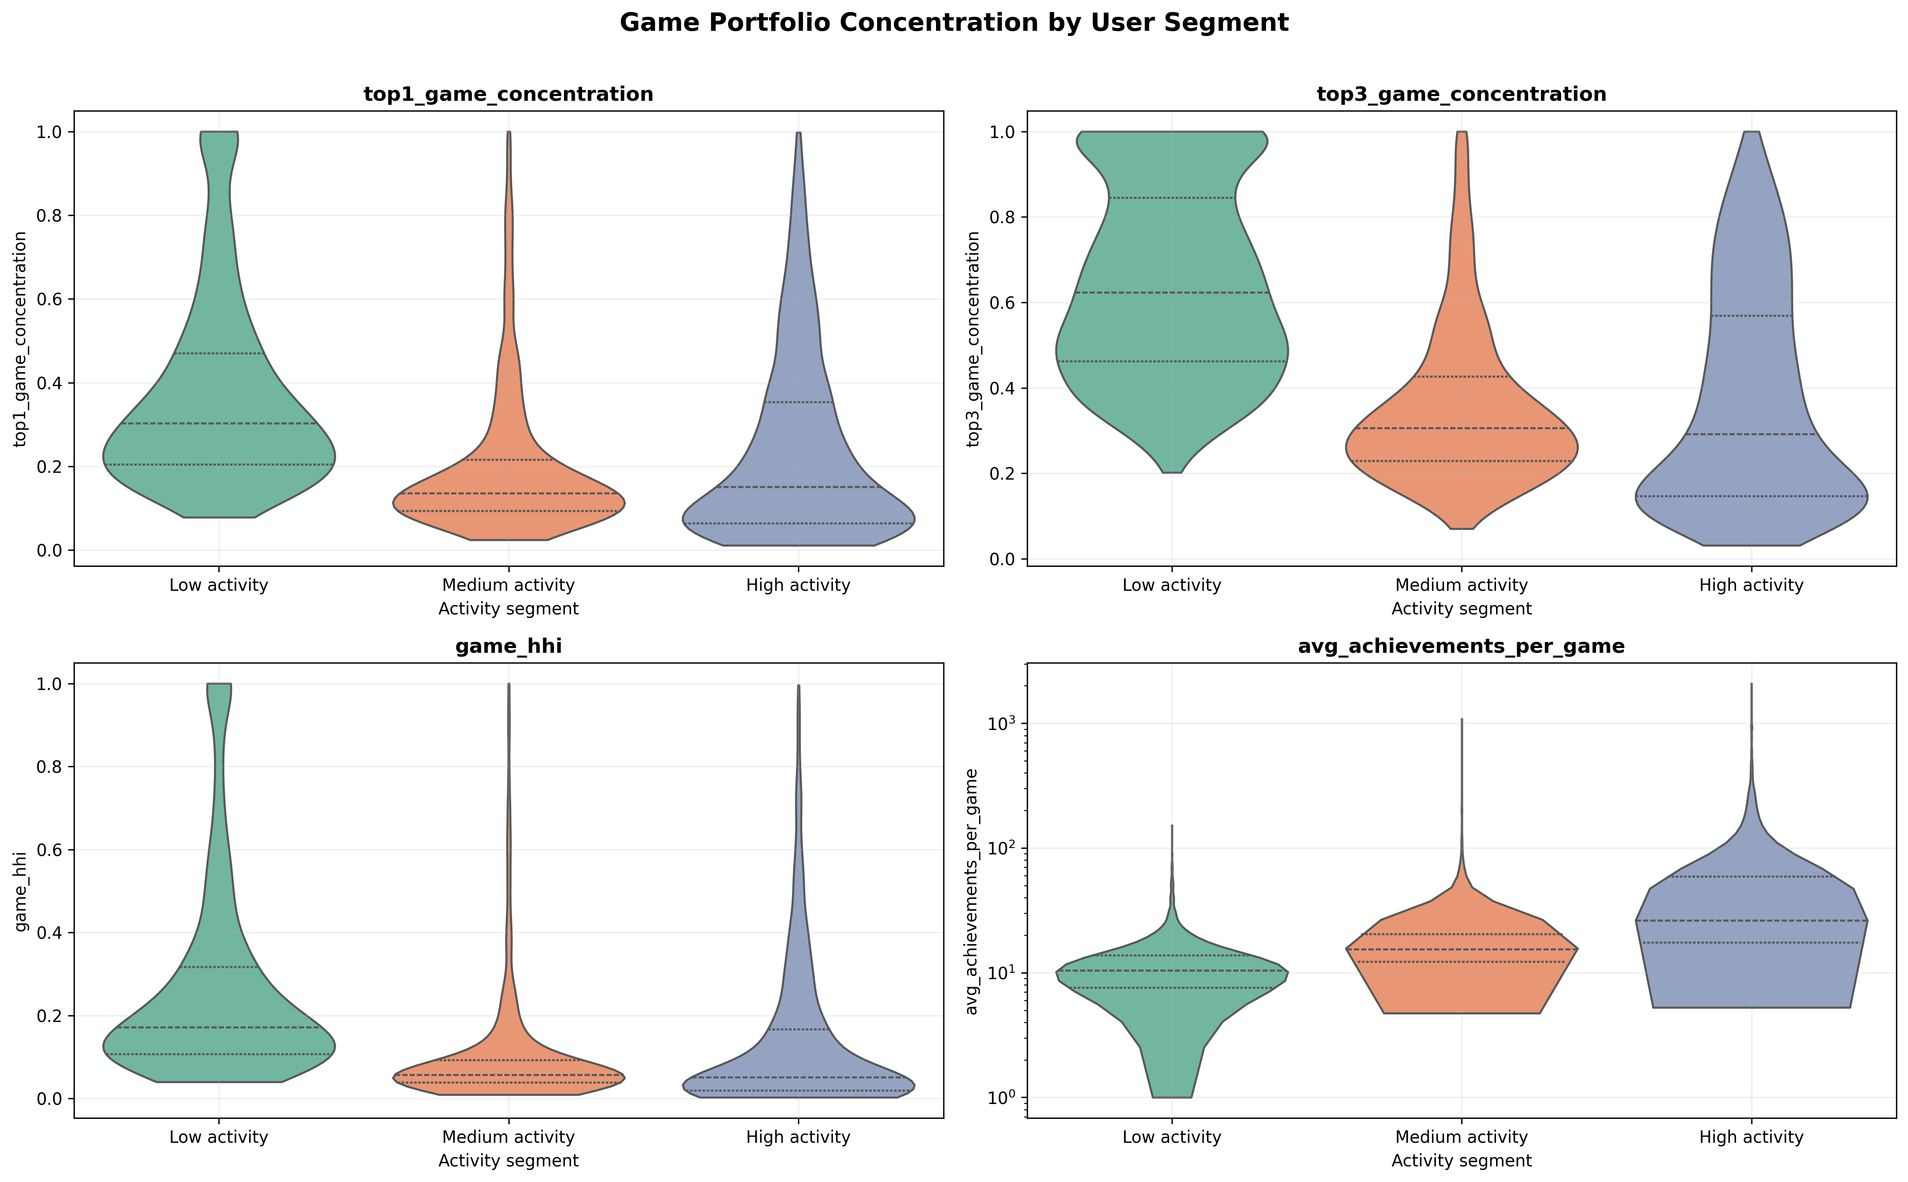
\includegraphics[width=0.7\linewidth]{Images/Slide/img151}
    }{
        \fbox{\begin{minipage}{0.7\linewidth}
            \centering
            \vspace{2cm}
            [IMAGE PLACEHOLDER]\\
            \texttt{Images/Slide/img151.jpg}\\
            \vspace{2cm}
        \end{minipage}}
    }
    \caption{Tầm quan trọng của các đặc trưng trong mô hình XGBoost}
    \label{fig:xgb_importance}
\end{figure}


Function \texttt{\_evaluate\_xgboost()}:

\begin{itemize}
    \item \textbf{PR-AUC}: 0.7252
    \item \textbf{ROC-AUC}: 0.9050
    \item \textbf{Optimal Threshold}: 0.9982 (F1-score tối ưu)
    \item \textbf{Classification Report (Bot class)}: Precision: 0.91, Recall: 0.66, F1-Score: 0.76
    \item Output plots:
    \begin{itemize}
        \item \texttt{xgb\_pr\_curve.png}: Đường cong Precision-Recall
        \item \texttt{xgb\_feature\_importance.png}: Biểu đồ tầm quan trọng đặc trưng
    \end{itemize}
\end{itemize}


\subsection{Phân Tích So Sánh Đặc Trưng}

\begin{itemize}
    \item So sánh: Top-50 flagged accounts vs Normal accounts
    \item Tính: Mean của mỗi đặc trưng trong 2 nhóm
    \item Output: \texttt{top50\_flagged\_profiles.csv} — profile trung bình của bot vs normal
    \item Giúp hiểu thành phần nào của feature matrix là discriminative nhất
\end{itemize}

\subsection{Phân Tích Khả Năng Giải Thích SHAP}

Giải thích độ đóng góp của từng đặc trưng đối với từng dự báo:

\begin{enumerate}
    \item \textbf{Sampling}: Chọn ngẫu nhiên 5000 hàng từ $X_{\text{raw}}$ (giữ thang đo gốc để dễ giải thích).
    \item \textbf{SHAP Calculation}: Tính SHAP values thông qua tính năng \texttt{pred\_contribs} của XGBoost.
    \item \textbf{Visualization}: Xuất các biểu đồ Summary, Waterfall và Scatter để phân tích tác động cục bộ và toàn cục.
\end{enumerate}

\begin{figure}[H]
    \centering
    \IfFileExists{Images/Slide/img156.jpg}{
        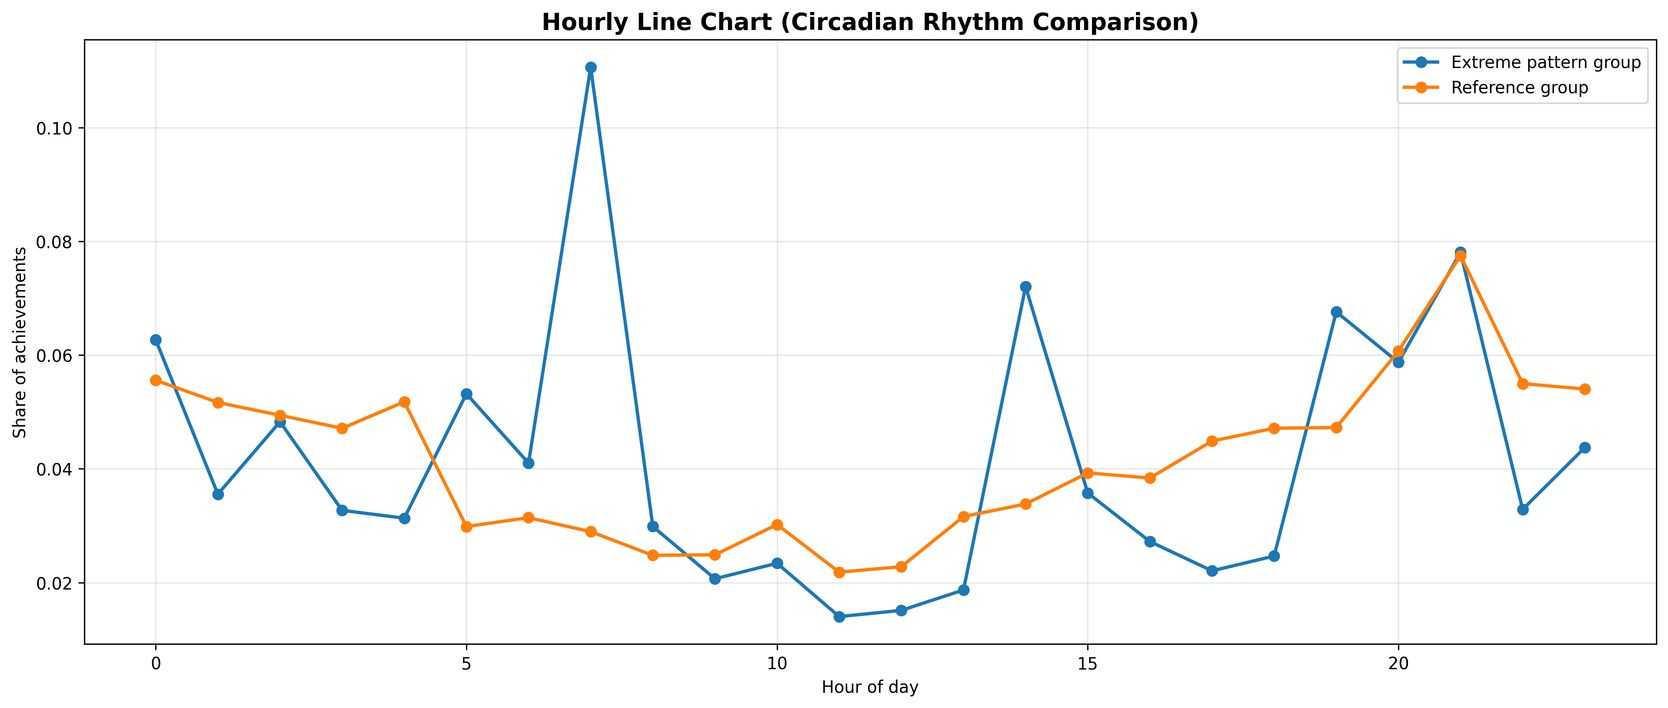
\includegraphics[width=0.7\linewidth]{Images/Slide/img156}
    }{
        \fbox{\begin{minipage}{0.7\linewidth}
            \centering
            \vspace{2cm}
            [IMAGE PLACEHOLDER]\\
            \texttt{Images/Slide/img156.jpg}\\
            \vspace{2cm}
        \end{minipage}}
    }
    \caption{Biểu đồ SHAP scatter thể hiện tác động của các giá trị đặc trưng}
    \label{fig:shap_scatter}
\end{figure}


\begin{figure}[H]
    \centering
    \IfFileExists{Images/Slide/img157.jpg}{
        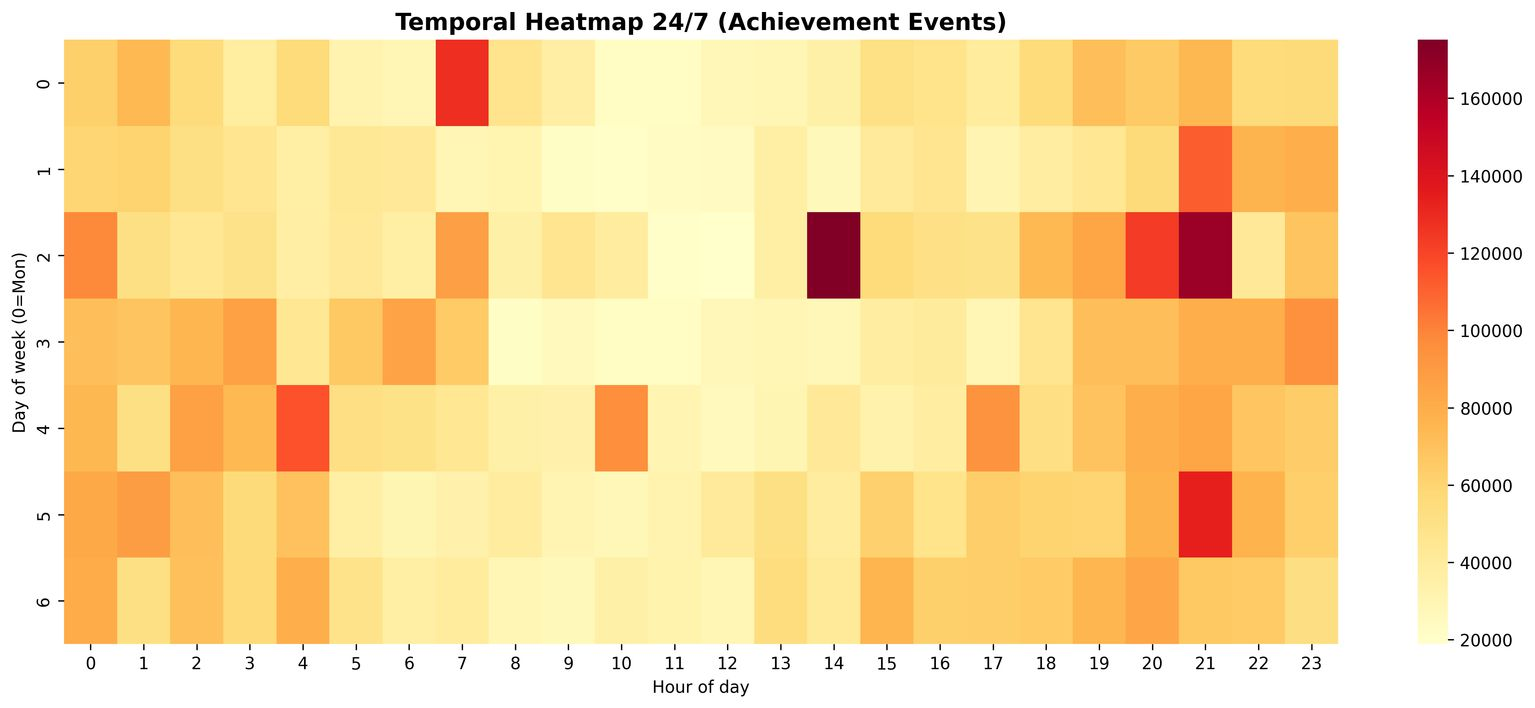
\includegraphics[width=0.7\linewidth]{Images/Slide/img157}
    }{
        \fbox{\begin{minipage}{0.7\linewidth}
            \centering
            \vspace{2cm}
            [IMAGE PLACEHOLDER]\\
            \texttt{Images/Slide/img157.jpg}\\
            \vspace{2cm}
        \end{minipage}}
    }
    \caption{Biểu đồ SHAP waterfall giải thích cho một trường hợp cụ thể}
    \label{fig:shap_waterfall}
\end{figure}


\section{Hệ Thống Dashboard BI}

Hệ thống cung cấp giao diện trực quan để theo dõi và phân tích các tài khoản bất thường.

\subsection{Giao Diện Tìm Kiếm và Truy Vấn}
Người dùng có thể tìm kiếm theo Steam ID hoặc tải lên danh sách file CSV/TXT.

\begin{figure}[H]
    \centering
    \IfFileExists{Images/Slide/img162.jpg}{
        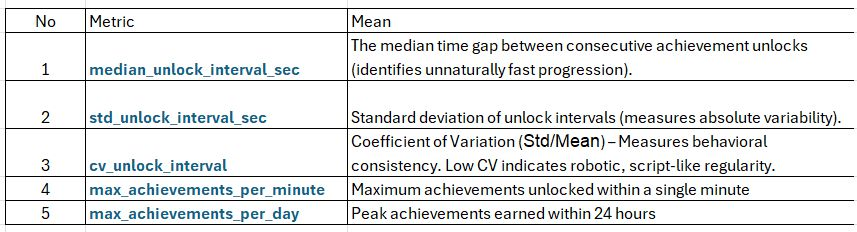
\includegraphics[width=0.7\linewidth]{Images/Slide/img162}
    }{
        \fbox{\begin{minipage}{0.7\linewidth}
            \centering
            \vspace{2cm}
            [IMAGE PLACEHOLDER]\\
            \texttt{Images/Slide/img162.jpg}\\
            \vspace{2cm}
        \end{minipage}}
    }
    \caption{Giao diện tìm kiếm tài khoản trên Dashboard}
    \label{fig:dash_search}
\end{figure}


\subsection{Chi Tiết Hành Vi và So Sánh Baseline}
Hệ thống hiển thị các chỉ số hành vi chi tiết so với mức trung bình của cộng đồng.

\begin{figure}[H]
    \centering
    \IfFileExists{Images/Slide/img167.jpg}{
        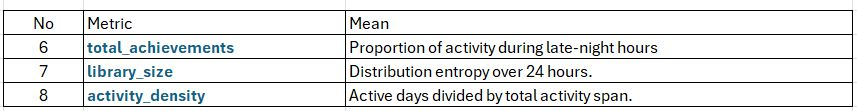
\includegraphics[width=0.7\linewidth]{Images/Slide/img167}
    }{
        \fbox{\begin{minipage}{0.7\linewidth}
            \centering
            \vspace{2cm}
            [IMAGE PLACEHOLDER]\\
            \texttt{Images/Slide/img167.jpg}\\
            \vspace{2cm}
        \end{minipage}}
    }
    \caption{Chi tiết các chỉ số hành vi của một tài khoản}
    \label{fig:dash_details}
\end{figure}


\begin{figure}[H]
    \centering
    \IfFileExists{Images/Slide/img172.jpg}{
        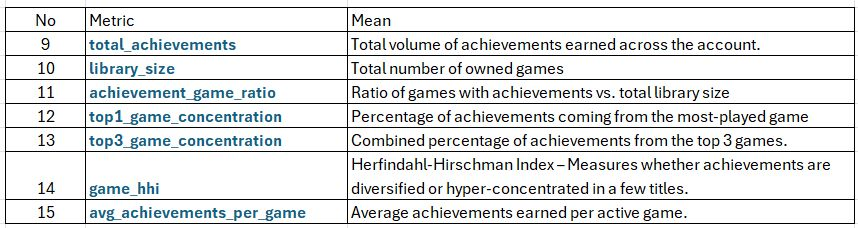
\includegraphics[width=0.7\linewidth]{Images/Slide/img172}
    }{
        \fbox{\begin{minipage}{0.7\linewidth}
            \centering
            \vspace{2cm}
            [IMAGE PLACEHOLDER]\\
            \texttt{Images/Slide/img172.jpg}\\
            \vspace{2cm}
        \end{minipage}}
    }
    \caption{So sánh 12 đặc trưng sai lệch nhất so với Baseline}
    \label{fig:comp_baseline}
\end{figure}


\subsection{Phân Tích Tổng Quan Dữ Liệu}

\begin{figure}[H]
    \centering
    \IfFileExists{Images/Slide/img177.jpg}{
        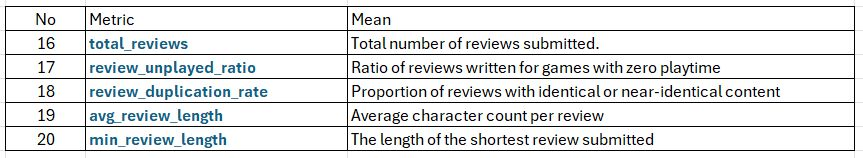
\includegraphics[width=0.7\linewidth]{Images/Slide/img177}
    }{
        \fbox{\begin{minipage}{0.7\linewidth}
            \centering
            \vspace{2cm}
            [IMAGE PLACEHOLDER]\\
            \texttt{Images/Slide/img177.jpg}\\
            \vspace{2cm}
        \end{minipage}}
    }
    \caption{Phân phối điểm Composite Score trong toàn bộ tập dữ liệu}
    \label{fig:dist_score}
\end{figure}


\begin{figure}[H]
    \centering
    \IfFileExists{Images/Slide/img182.jpg}{
        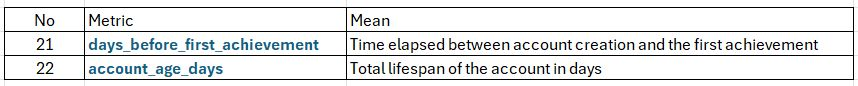
\includegraphics[width=0.7\linewidth]{Images/Slide/img182}
    }{
        \fbox{\begin{minipage}{0.7\linewidth}
            \centering
            \vspace{2cm}
            [IMAGE PLACEHOLDER]\\
            \texttt{Images/Slide/img182.jpg}\\
            \vspace{2cm}
        \end{minipage}}
    }
    \caption{Phân bố địa lý của các tài khoản bất thường}
    \label{fig:geo_dist}
\end{figure}

\begin{figure}[H]
    \centering
    \IfFileExists{Images/Slide/img183.jpg}{
        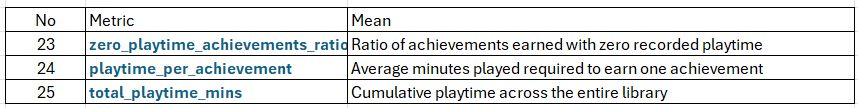
\includegraphics[width=0.7\linewidth]{Images/Slide/img183}
    }{
        \fbox{\begin{minipage}{0.7\linewidth}
            \centering
            \vspace{2cm}
            [IMAGE PLACEHOLDER]\\
            \texttt{Images/Slide/img183.jpg}\\
            \vspace{2cm}
        \end{minipage}}
    }
    \caption{Tương quan mô hình và Dashboard đồng thuận Ensemble}
    \label{fig:dash_consensus}
\end{figure}


\begin{figure}[H]
    \centering
    \IfFileExists{Images/Slide/img197.jpg}{
        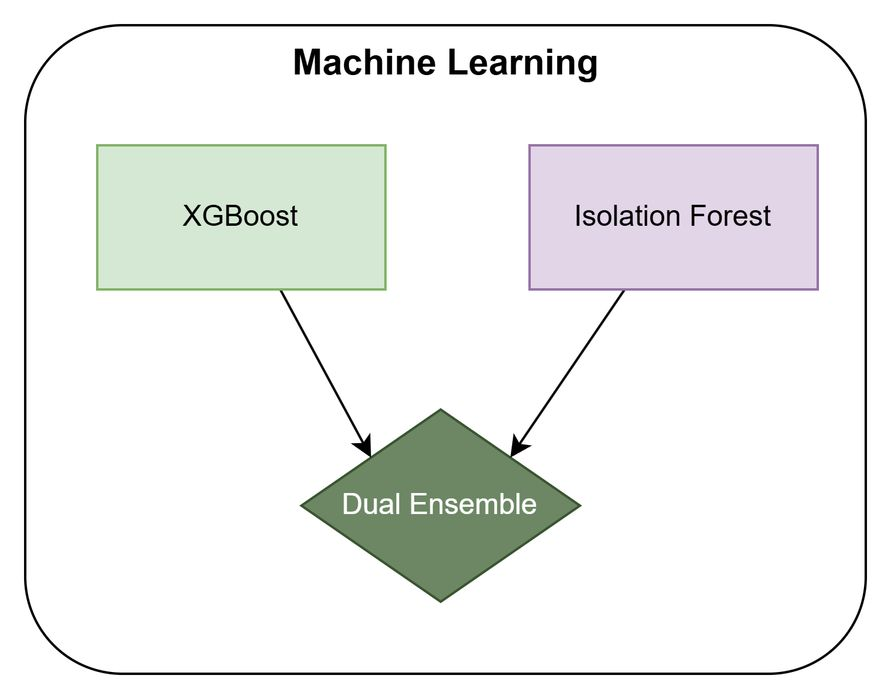
\includegraphics[width=0.7\linewidth]{Images/Slide/img197}
    }{
        \fbox{\begin{minipage}{0.7\linewidth}
            \centering
            \vspace{2cm}
            [IMAGE PLACEHOLDER]\\
            \texttt{Images/Slide/img197.jpg}\\
            \vspace{2cm}
        \end{minipage}}
    }
    \caption{Ma trận đồng thuận giữa XGBoost và Isolation Forest}
    \label{fig:consensus}
\end{figure}


\subsection{Phân Tích Đặc Trưng Discriminative}

\begin{figure}[H]
    \centering
    \IfFileExists{Images/Slide/img206.jpg}{
        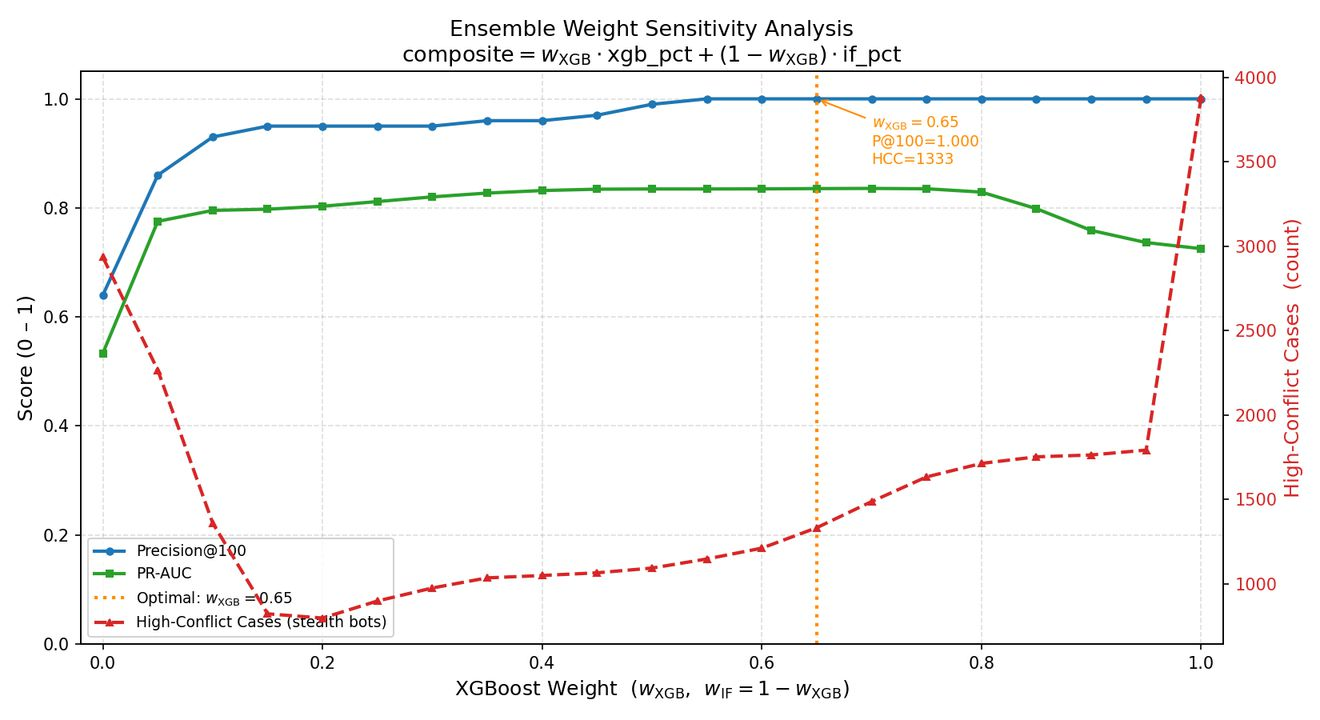
\includegraphics[width=0.7\linewidth]{Images/Slide/img206}
    }{
        \fbox{\begin{minipage}{0.7\linewidth}
            \centering
            \vspace{2cm}
            [IMAGE PLACEHOLDER]\\
            \texttt{Images/Slide/img206.jpg}\\
            \vspace{2cm}
        \end{minipage}}
    }
    \caption{So sánh tỷ lệ và chỉ số Cohen's d giữa nhóm Bot và Normal}
    \label{fig:effect_size}
\end{figure}


\begin{figure}[H]
    \centering
    \IfFileExists{Images/Slide/img211.jpg}{
        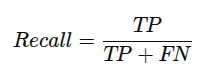
\includegraphics[width=0.7\linewidth]{Images/Slide/img211}
    }{
        \fbox{\begin{minipage}{0.7\linewidth}
            \centering
            \vspace{2cm}
            [IMAGE PLACEHOLDER]\\
            \texttt{Images/Slide/img211.jpg}\\
            \vspace{2cm}
        \end{minipage}}
    }
    \caption{Tương quan giữa độ tuổi tài khoản và hoạt động đánh giá}
    \label{fig:corr_behavior}
\end{figure}


\begin{figure}[H]
    \centering
    \IfFileExists{Images/Slide/img212.jpg}{
        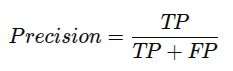
\includegraphics[width=0.45\linewidth]{Images/Slide/img212}
        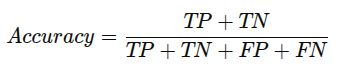
\includegraphics[width=0.45\linewidth]{Images/Slide/img213} \\
        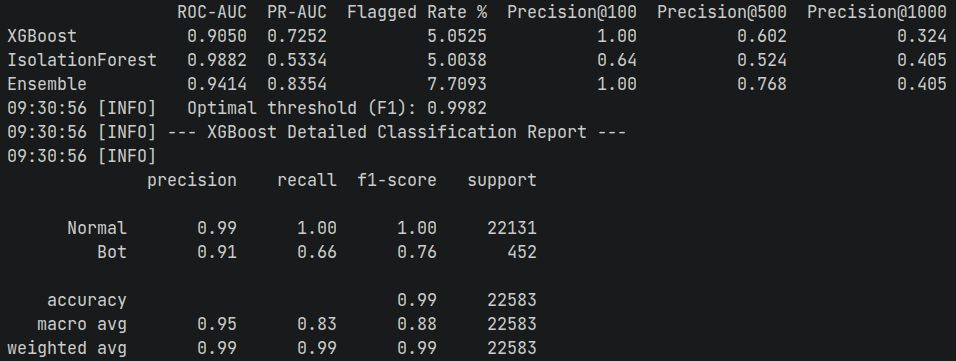
\includegraphics[width=0.45\linewidth]{Images/Slide/img218}
        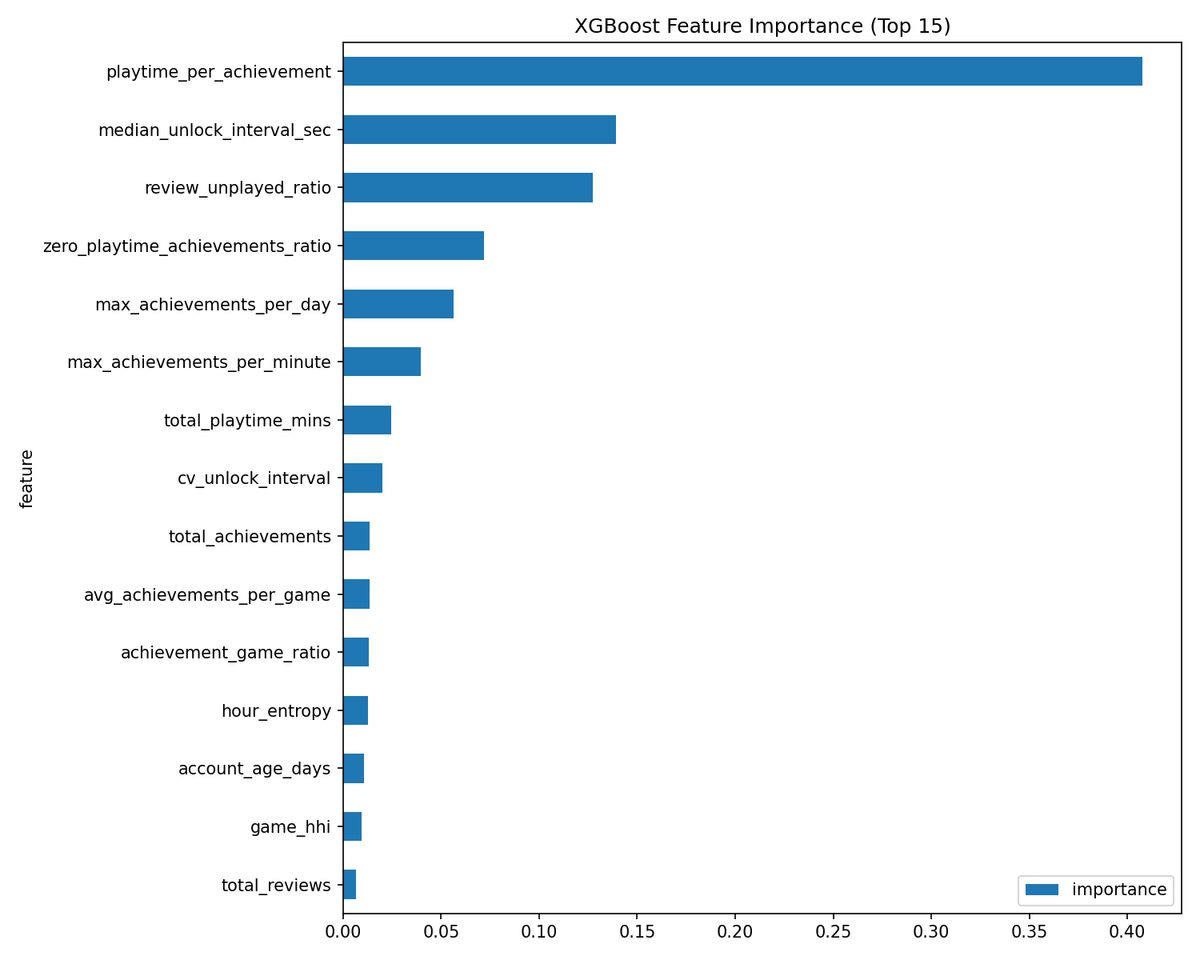
\includegraphics[width=0.45\linewidth]{Images/Slide/img223}
    }{
        \fbox{\begin{minipage}{0.7\linewidth}
            \centering
            \vspace{2cm}
            [IMAGE PLACEHOLDER]\\
            \texttt{Images/Slide/img212.jpg - img309.jpg}\\
            \vspace{2cm}
        \end{minipage}}
    }
    \caption{Tỷ lệ bất thường theo quy mô thư viện, thời gian chơi và năm tạo tài khoản}
    \label{fig:anomaly_rates}
\end{figure}



\section{Cải Tiến Liên Tục}

\subsection{Chu Kỳ}
\begin{enumerate}
    \item \textbf{Inference}: Dự báo trên dữ liệu mới
    \item \textbf{Active Learning}: Tạo mẫu conflict cho human review
    \item \textbf{Human Labeling}: Reviewer gán nhãn
    \item \textbf{Re-training}: Integrate human labels → train mô hình lại
    \item \textbf{Evaluation}: Đánh giá chất lượng → quay lại bước 1
\end{enumerate}

\subsection{Metrics Theo Dõi}
\begin{itemize}
    \item \textbf{ROC-AUC}: Không còn auto-flip; log để theo dõi chất lượng
    \item \textbf{PR-AUC}: Metric chính cho imbalanced data
    \item \textbf{Precision@Top-K}: Độ chính xác trong top-K suspicious accounts (K = 100, 500, 1000)
    \item \textbf{Human Agreement Rate}: Tỷ lệ mô hình dự báo đúng với human labels
\end{itemize}

\section{Tóm Tắt}
Giai đoạn dự báo \& ứng dụng bao gồm: (1) Inference trên dữ liệu mới, (2) Active Learning để xác định mẫu cần review, (3) Human-in-the-Loop labeling để cải thiện, (4) Đánh giá toàn diện chất lượng mô hình qua 4 nhóm metrics, (5) Chu kỳ cải tiến liên tục. Hệ thống được thiết kế để tăng độ chính xác \& độ tin cậy theo thời gian thông qua feedback từ human reviewers.
``

\section{Tóm Tắt}
Hệ thống không chỉ dừng lại ở dự báo tĩnh, mà còn đưa ra cấu trúc học tập vòng lặp (Active Learning) nhờ human-in-the-loop, bảo đảm mô hình ngày càng chính xác theo thời gian.
